\chapter{The possibilities of AR in remote collaboration }
\label{secMainPart}
\section{The possibilities of AR in remote collaboration}
The current standard for remote video conferencing are tools like Zoom, where all participants get recorded by a webcam and a microphone, and they communicate only through these mediums. This approach comes with many downsides. Firstly, the social presence with 2d video conferencing is very low, which leads to many problems. From an efficiency standpoint, higher social presence leads to improved task performance and time efficiency as discussed in the paper "Social interaction in augmented reality" \cite{10.1371/journal.pone.0216290} due to social facilitation. This means that with lower social presence from other participants, workers tend to perform worse and will not be as productive. Secondly, with increased social presence comes better working morale from the participants, because with many workers switching to home office came a greater feeling of social isolation \cite{joitmc7010070}. 
This impacts the workers' mental health negatively and worsens their performance and well-being. Again, by implementing AR into remote collaboration, the social presence will be improved and these problems will be solved. Through AR the social presence is increased, because it allows for Three-dimensional video conferencing which, as Hauber et al. found, increases social presence significantly \cite{2dSocialPresence}. Another study by Doherty-Sneddon et Al. \cite{taskPerformance} found that task efficiency 2d video communication is worse than face-to-face, meaning that it takes more words to transmit information in video communication than in face-to-face communication. This is mostly due to the fact that the visual signals it provided didn't help listeners understand in the same way as visual signals in face-to-face interaction did. Another important nonverbal cue that is missing in 2d-video-communication is eye-contact. Although eye contact is not necessary for the task to be completed successfully, it may have a significant impact on how satisfying the communicative experience is for users. This, again, leads to a reduction in efficiency and productivity of workers, while increasing the feeling of isolation because eye contact leads to greater sympathy between two collaborators.
\begin{figure}[H]
\centering
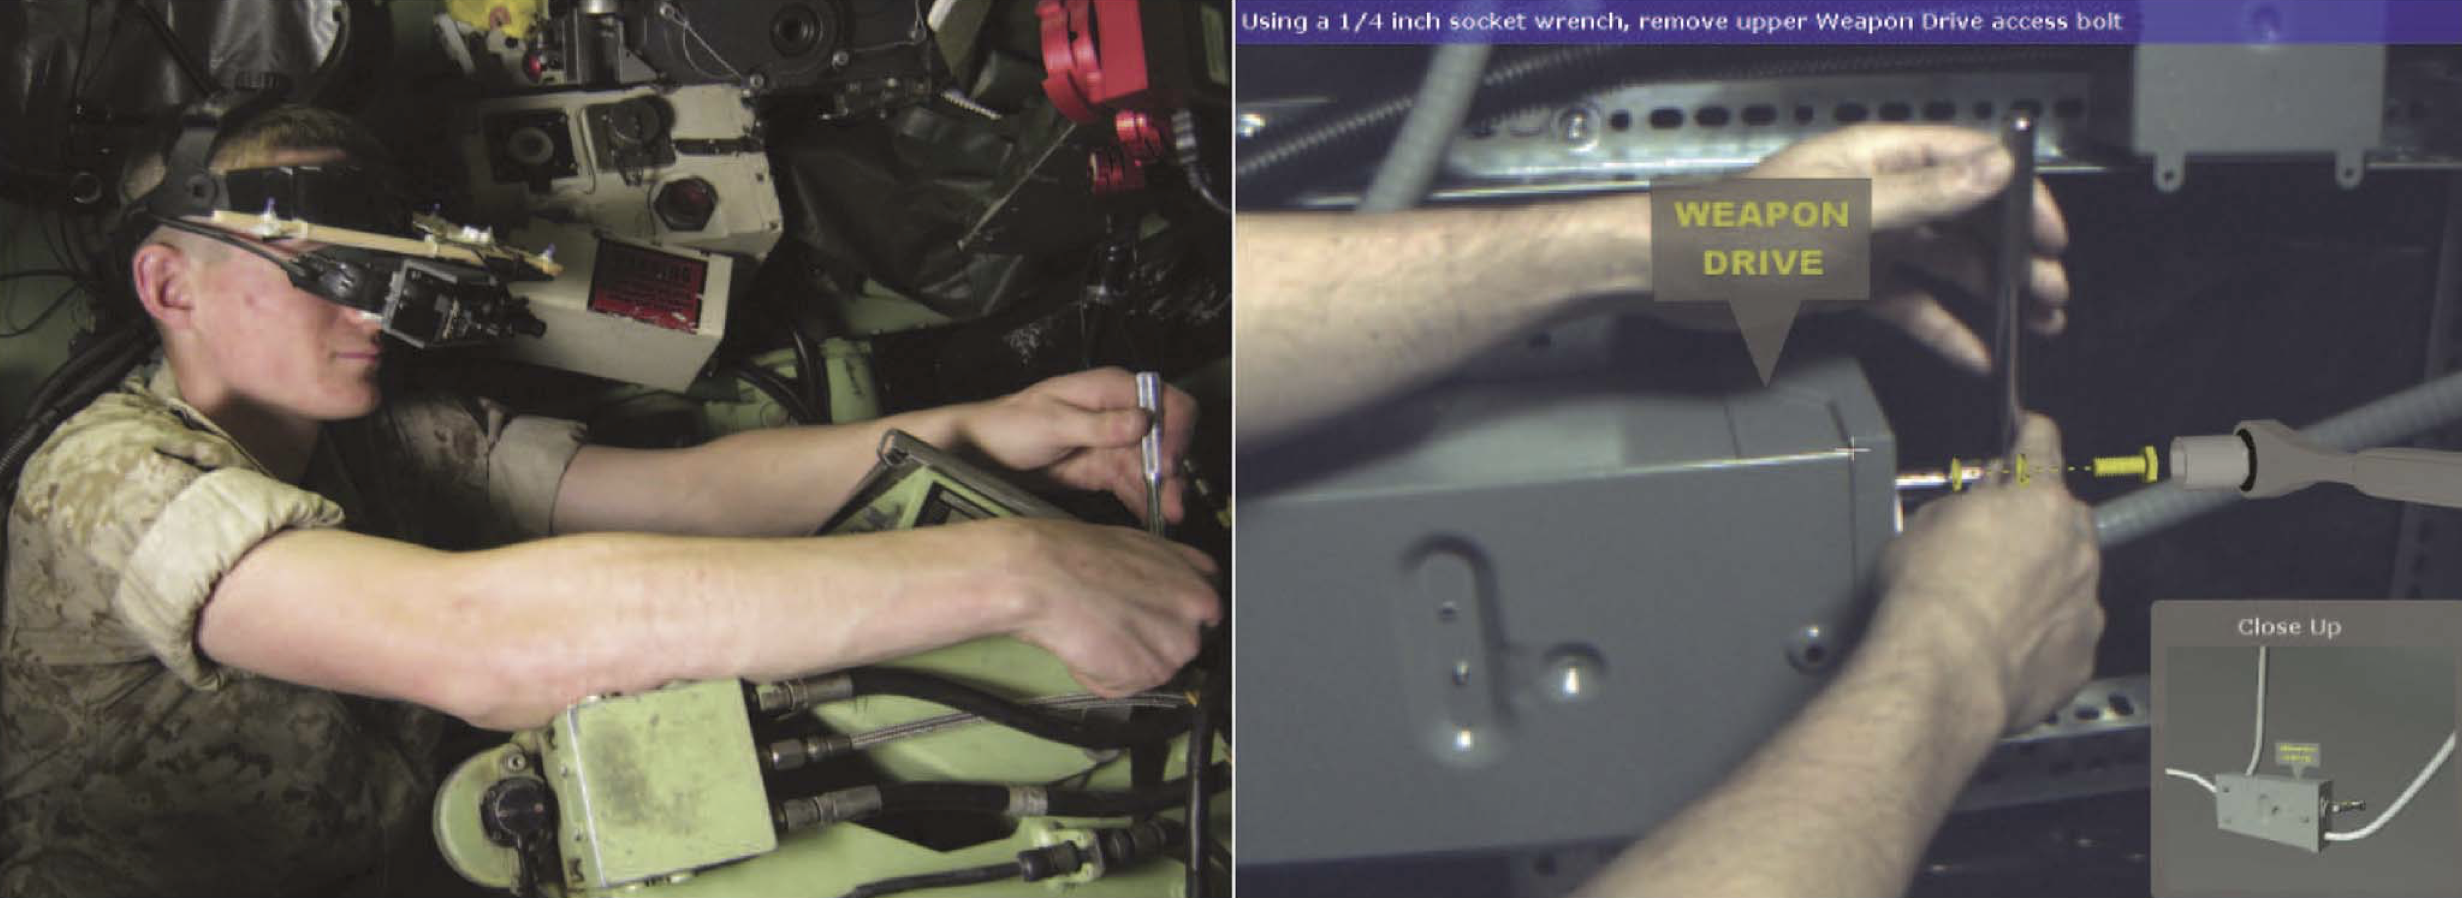
\includegraphics[width = 0.8\textwidth]{figures/ARmaintenance}
\caption[test]{(Left) A mechanic wearing a tracked headworn display removes a bolt from a component inside an armored personnel carrier turret. (Right) A view through the AR display virtually superimposing information onto the real world}
\label{fig::maintenance}
\end{figure}

Furthermore, when working on real-world problems like maintenance where fast problem-solving is required if some problem occurs, expert opinions play an important role. Because these problems have to be solved in the real world, they often cannot show up in person and have to collaborate remotely through video conferencing. This can lead to dramatically less efficient communication when trying to solve this problem remotely, because, as Billinghurst et al. concluded in their study, discussing real-world objects through 2D video conferencing is inefficient because non-verbal communication like pointing is crucial for intuitive collaboration \cite{CollaborativeAR}. AR offers the possibility of having a remote collaborator, represented by a virtual agent, projected onto the real world. This allows for remote collaboration that feels to both users like intuitive face-to-face collaboration and allows for more efficient workflows. Furthermore, information regarding the real-world objects can be superimposed onto them using AR as seen in \ref{fig::maintenance}, which makes the process much better because it enhances the efficiency of maintenance, especially with complex parts \cite{5620905}.

\section{Optimal Avatar design}
An important choice to make is the avatar design, because it greatly affects the perceived social presence of the avatar for the user as discussed in \ref{effectOfAvatarAppearance}. However, the optimal design choices for the avatar's appearance differ between distinct use cases, which makes it important to explore how different design choices affect the users' perception of the avatar.

The first important decision is the appearance of the Avatar. depending on the use case, different appearances can have different effects on the user. In general, it can be said that the more realistic the avatar, the better the interaction and the social connectedness. Latoschik et al. \cite{avatarRealism} found that a more realistic avatar finds better acceptance in users which leads to a better connectedness in collaboration. However, under certain circumstances, the study found that participants experienced an uncanny valley effect where if the avatar imperfectly resembles a realistic human being, the observers experienced a feeling of uneasiness and revulsion \cite{8797719}. 

\begin{figure}[H]
\centering
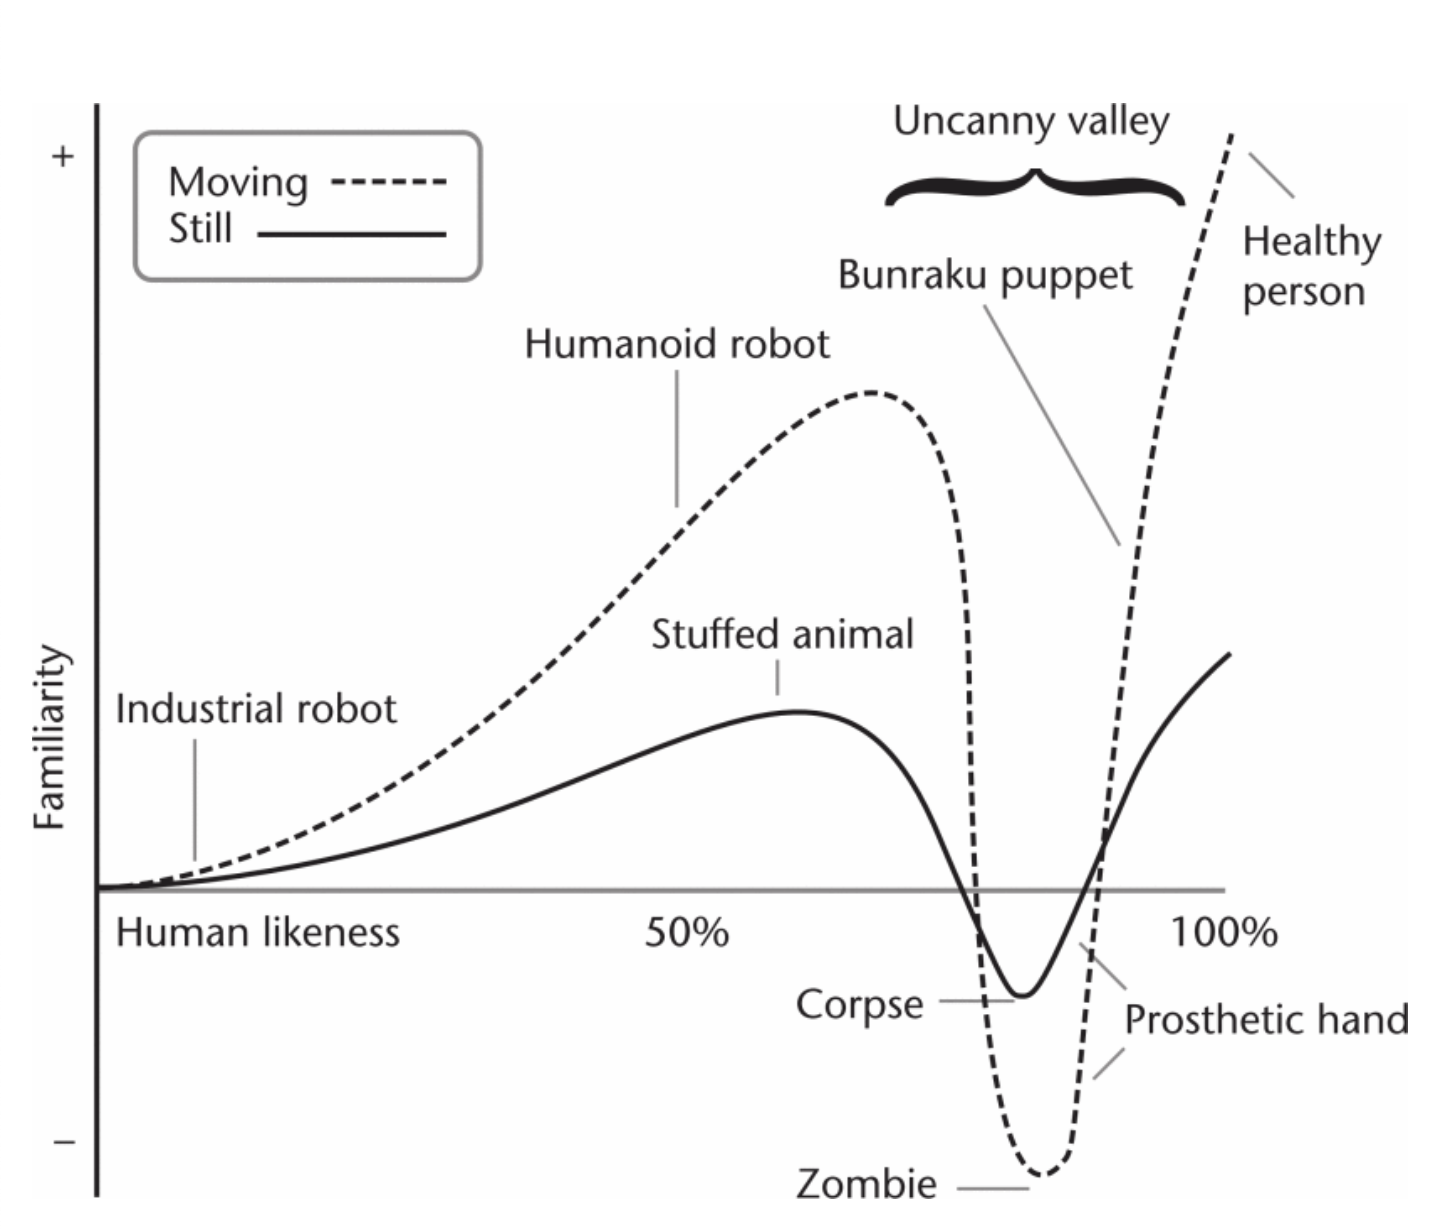
\includegraphics[width = 0.5\textwidth]{figures/uncannyValley}
\caption[Study 1 setup]{Visual representation of the uncanny valley effect}
\label{fig::uncannyValley}
\end{figure}

The uncanny valley effect is a controversial phenomenon that occurs when human or humanlike characters fail to arouse our sympathy and rather cause discomfort in the observer, even if it resembles a human closely. This means that when virtual characters approach realistic similarity to humans while still having imperfections, they become eerie or frightening. But when these similarities are perfected, the characters suddenly become very familiar again as seen in \ref{fig::uncannyValley}. \cite{4557950}

Due to these effects, it is important to take the computing power of the device in use into consideration: when rendering a realistic avatar, even small imperfections lead to great discomfort and uneasiness in users. This shows further research potential in this field, because with improved graphics the appearance of the avatar can be improved to better resemble realistic humans, which opens the possibility of overcoming the uncanny valley effect and having a greater distinction between cartoon and realistic avatars.

As Yoon et al. found in their studies, social Presence was highest with avatars that were realistic and where the whole body was visible, although, as already discussed, it resulted in an uncanny feeling in some participants. In general, Whole-body avatars were perceived as the most present, with avatars consisting of only the upper body getting positive recognition as well \cite{8797719}. This means that for remote collaboration, the avatar or virtual agent should at least be consisting of an upper body to feel natural to the user. 

\begin{figure}[H]
\centering
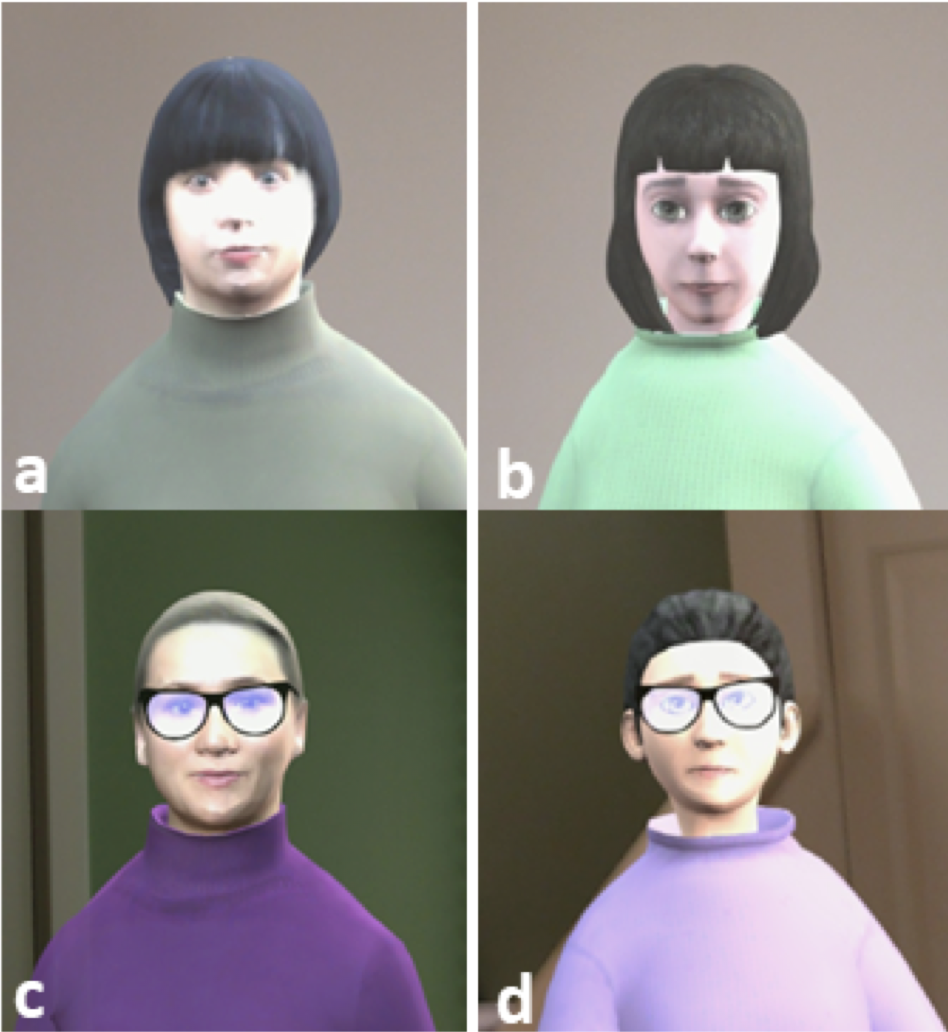
\includegraphics[width = 0.5\textwidth]{figures/Bildschirmfoto 2022-06-10 um 19.48.36}
\caption[Study 1 setup]{Example of realistic (a,c) and cartoon (b,d) avatar upper bodies}
\label{fig::solutions}
\end{figure}

Other studies at Microsoft from C. Dobre et al. \cite{Microsoft} concluded as well that a realistic appearance has better perceived nonverbal behavior and felt more appropriate to the participants than a cartoon avatar. This is especially interesting because the study was conducted in a working space, so it underlined the previous statements about their usefulness in work meetings. However, the study also found that the appearance of avatars got less important with time, meaning that the participants got accustomed to the avatars' appearance, no matter if realistic or cartoonish. Further work could elaborate on this study and test the reaction of younger participants to cartoon or realistic avatars. This way the perceived friendliness can be differentiated by testing different age groups and the most appropriate avatars for applications at schools or nursing homes can be found. Additionally, with improving technology it may be possible to improve the realism of the realistic avatars and remodel the cartoon avatars to be more appealing to children.

This does not mean however that cartoon characters do not have applications, because in general, while the realistic avatar was perceived as best for efficient collaboration and social presence, the cartoon characters gave the participants a sense of comfort and friendliness, as well as having the benefit of no uncanny valley \cite{8797719}. This means that realistic whole-body avatars are the best for collaborative environments, but cartoon whole-body or upper-body avatars are suited better for applications involving children or in general outside of the working environment.
